\documentclass[french,a4paper,10pt]{article}

\usepackage[a4paper,hmargin=30mm,vmargin=30mm]{geometry}
\usepackage[T1]{fontenc} % font type
\usepackage[french]{babel} % language
\usepackage{lmodern} % font type
\usepackage[shortlabels]{enumitem}
\usepackage{hyperref}
\usepackage{graphicx}
\usepackage{sectsty}
%\setlength{\parindent}{0pt}



\title{Compte Rendu TP1\\Prise en main d'une libraire de traitement d'images}
\author{Ivan Lejeune}
\date{\today}


\begin{document}

	\maketitle

	% make table of contents
	\tableofcontents

	\newpage
	\section{Seuillage d'une image au format pgm}\label{sec:1}

	\subsection{Ouverture des fichiers}\label{subsec:1.1}
	On commence par t\'el\'echarger les fichiers se trouvant \'a
	\url{https://www.lirmm.fr/~wpuech/enseignement/donnees_multimedia/librairie/}.
	Ensuite, on les ouvre dans l'\'editeur de texte voulu, dans notre cas, on se servira de \emph{CLion}
	(et parfois de \emph{VSCodium}).
	
	\subsection{Téléchargement des fichiers nécessaires}\label{subsec:1.2}

	On t\'el\'echarge les fichiers depuis \url{https://www.lirmm.fr/~wpuech/enseignement/donnees_multimedia/images/}.

	C'est parmi ces images qu'on effectuera la majorit\'e du travail, notamment avec \emph{08.pgm} et \emph{peppers.pgm}.

	\subsection{Compilation, ex\'ecution et test}\label{subsec:1.3}

	On commence par assurer d'avoir plac\'e les fichiers \texttt{test\_grey.cpp} et \texttt{image\_pgm.cpp} dans le
	m\^eme r\'epertoire.

	On compile le programme \texttt{test\_grey.cpp} avec un seuil de 80 pour passer de l'image de gauche à celle de
	droite :
	\begin{figure}[!htb]
		\begin{minipage}{0.48\textwidth}
			\centering
			\fbox{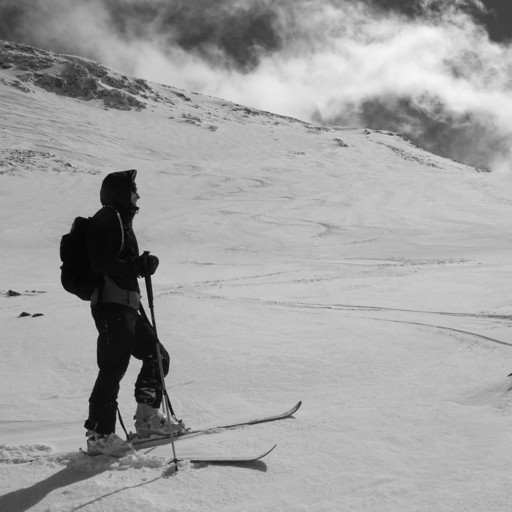
\includegraphics[width=.7\linewidth]{./out/orig-08}}
			\caption{Image originale}\label{Fig:orig-08}
		\end{minipage}\hfill
		\begin{minipage}{0.48\textwidth}
			\centering
			\fbox{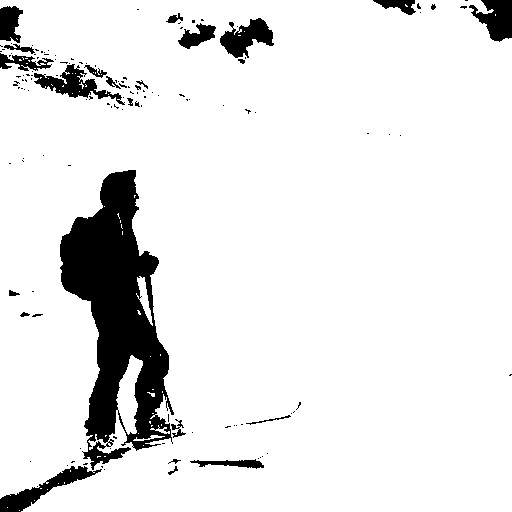
\includegraphics[width=.7\linewidth]{./out/test-grey-08}}
			\caption{Image modifiée avec un seuil de 80}\label{Fig:test-grey-08}
		\end{minipage}
	\end{figure}
	\newpage
	\section{Seuillage d'une image pgm avec plusieurs niveaux}\label{sec:2}

	\subsection{Seuillage en 3 parties}\label{subsec:2.1}
	On reprend le programme \texttt{test\_grey.cpp} pour le modifier afin de pouvoir effectuer un seuillage en 3
	parties.
	Il suffit de rajouter deux seuils supplémentaires, S2 et S3, et de les appliquer à l'image.
	Ici, on a pris des seuils à 80, 140 et 200 pour obtenir la transformation suivante :
	\begin{figure}[!htb]
		\begin{minipage}{0.48\textwidth}
			\centering
			\fbox{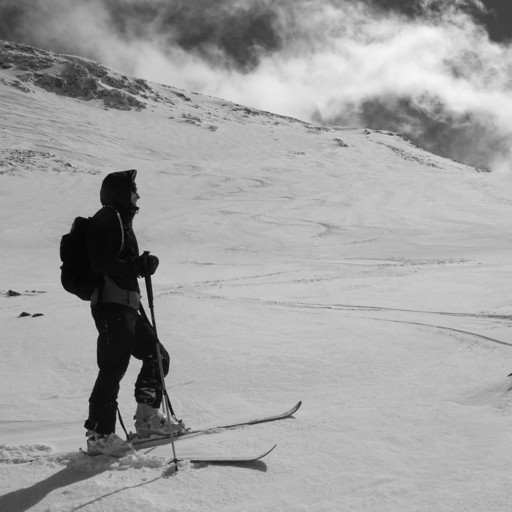
\includegraphics[width=.7\linewidth]{./out/orig-08}}
			\caption{Image originale}\label{Fig:orig-08-2}
		\end{minipage}\hfill
		\begin{minipage}{0.48\textwidth}
			\centering
			\fbox{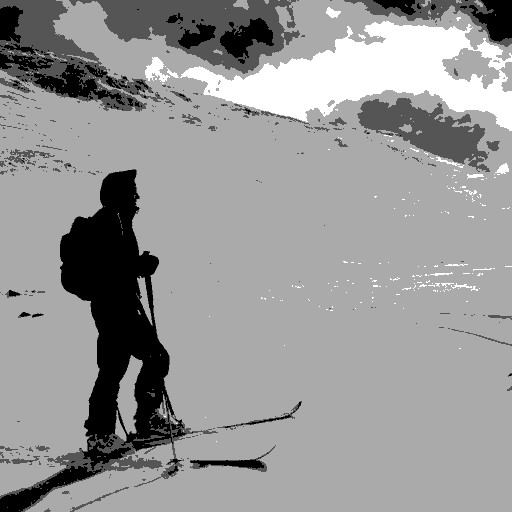
\includegraphics[width=.7\linewidth]{./out/test-grey-08-03}}
			\caption{Image modifiée avec 3 seuils}\label{Fig:test-grey-08-3}
		\end{minipage}
	\end{figure}

	\subsection{Seuillage en 4 parties}\label{subsec:2.2}
	On reprend le programme \texttt{test\_grey.cpp} pour le modifier afin de pouvoir effectuer un seuillage en 4
	parties.
	Il suffit de rajouter un seuil supplémentaire, S4, et de l'appliquer à l'image.
	Ici, on a pris des seuils à 40, 100, 160 et 220 pour obtenir la transformation suivante :
	\begin{figure}[!htb]
		\begin{minipage}{0.48\textwidth}
			\centering
			\fbox{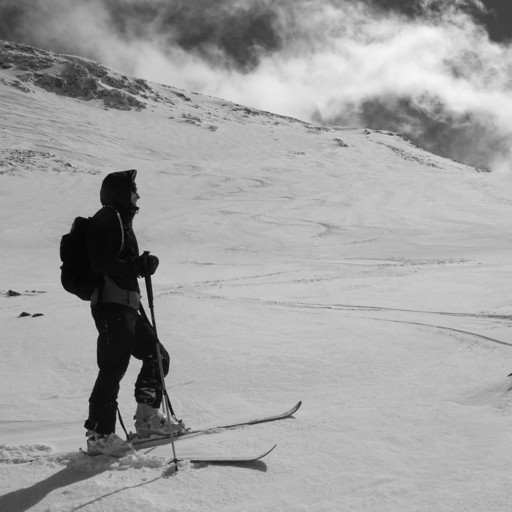
\includegraphics[width=.7\linewidth]{./out/orig-08}}
			\caption{Image originale}\label{Fig:orig-08-3}
		\end{minipage}\hfill
		\begin{minipage}{0.48\textwidth}
			\centering
			\fbox{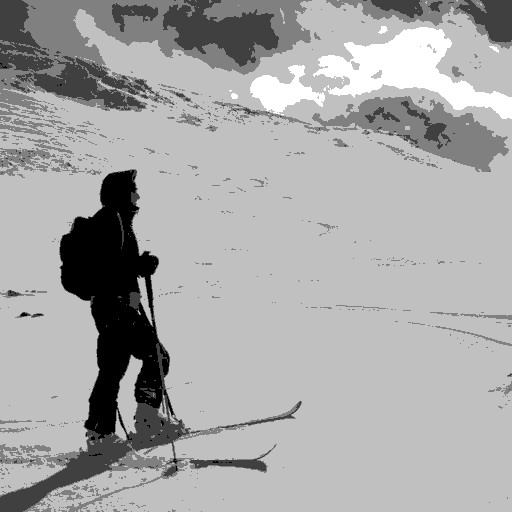
\includegraphics[width=.7\linewidth]{./out/test-grey-08-04}}
			\caption{Image modifiée avec 4 seuils}\label{Fig:test-grey-08-4}
		\end{minipage}
	\end{figure}

	\newpage
	\section{Histogramme d'une image pgm}\label{sec:3}

	\subsection{D\'eveloppement du programme}\label{subsec:3.1}

	Pour cette partie, on a d\'evelopp\'e un programme \texttt{histo.cpp} qui permet de g\'en\'erer l'histogramme
	d'une image pgm.
	Les données sont d'abord affichées dans la console, puis on les enregistre dans un fichier \texttt{histo.dat} pour
	pouvoir les visualiser avec \emph{gnuplot}.
	Le nom du fichier de sortie peut être rajouté en argument lors de l'exécution du programme.

	L'essentiel du code est le suivant : % insertion en image du code
	\begin{figure}[!htb]
		\centering
		\fbox{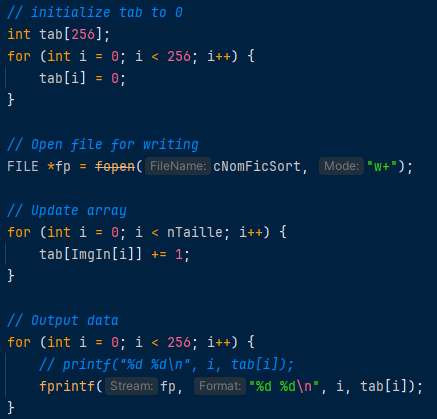
\includegraphics[width=.7\linewidth]{./out/histo-code}}
		\caption{Code de \texttt{histo.cpp}}\label{Fig:histo-code}
	\end{figure}

	\subsection{R\'esultats}\label{subsec:3.2}

	On a utilis\'e l'image \emph{08.pgm} pour tester le programme. Cela donne les r\'esultats suivants :
	% insert image of data file then of the histogram
	\begin{figure}[!htb]
		\begin{minipage}{0.48\textwidth}
			\centering
			% adjust image with height instead of width
			\fbox{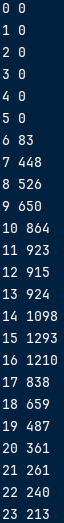
\includegraphics[height=0.7\linewidth]{./out/histo-data}}
			\caption{Donn\'ees de l'histogramme}\label{Fig:histo-data}
		\end{minipage}\hfill
		\begin{minipage}{0.48\textwidth}
			\centering
			\fbox{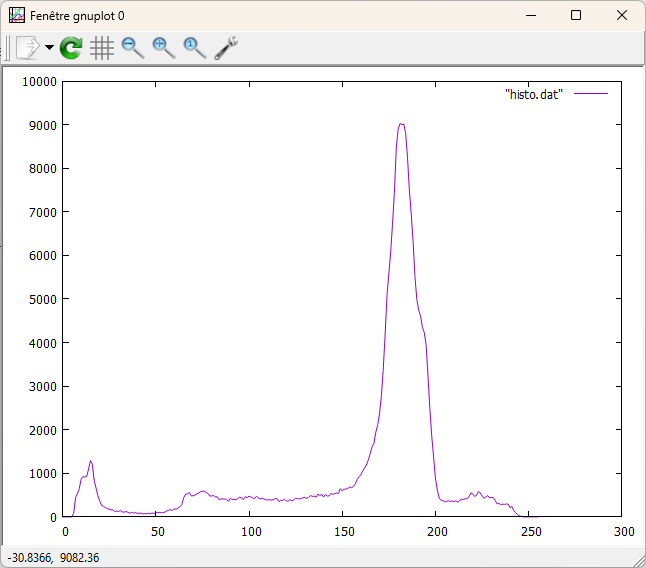
\includegraphics[width=.7\linewidth]{./out/histo-plot}}
			\caption{Histogramme de l'image}\label{Fig:histo-plot}
		\end{minipage}
	\end{figure}

	\newpage
	\section{Profil d'une ligne ou d'une colonne d'une image pgm}\label{sec:4}
	On a d\'evelopp\'e un programme \texttt{profil.cpp} qui permet de g\'en\'erer le profil d'une ligne ou d'une
	colonne d'une image pgm.
	Les donn\'ees sont d'abord affich\'ees dans la console, puis on les enregistre dans un fichier \texttt{profil.dat}
	pour pouvoir les visualiser avec \emph{gnuplot}.
	Le nom du fichier de sortie peut \^etre rajout\'e en argument lors de l'ex\'ecution du programme.

	L'essentiel du code est le suivant : % insertion en image du code
	\begin{figure}[!htb]
		\centering
		\fbox{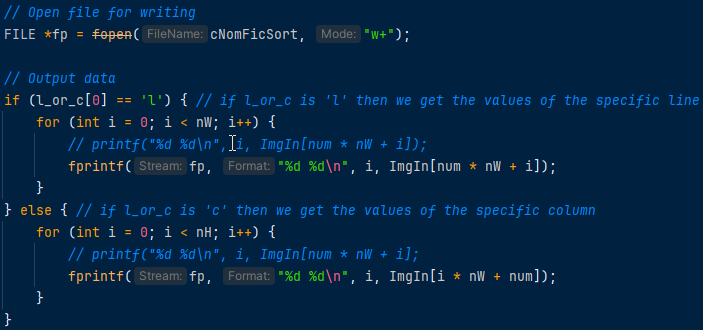
\includegraphics[width=.7\linewidth]{./out/profil-code}}
		\caption{Code de \texttt{profil.cpp}}\label{Fig:profil-code}
	\end{figure}

	\subsection{R\'esultats}\label{subsec:4.1}

	On a utilis\'e l'image \emph{08.pgm} pour tester le programme sur la 200-ième ligne.
	Cela donne les r\'esultats suivants :
	% insert image of data file then of the histogram
	\begin{figure}[!htb]
		\begin{minipage}{0.48\textwidth}
			\centering
			% adjust image with height instead of width
			\fbox{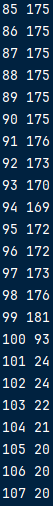
\includegraphics[height=0.7\linewidth]{./out/profil-data}}
			\caption{Donn\'ees de l'histogramme}\label{Fig:profil-data}
		\end{minipage}\hfill
		\begin{minipage}{0.48\textwidth}
			\centering
			\fbox{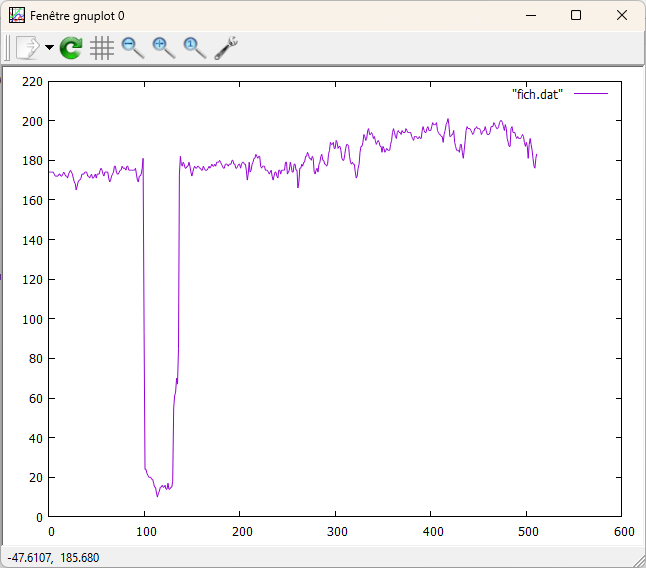
\includegraphics[width=.7\linewidth]{./out/profil-plot}}
			\caption{Histogramme de l'image}\label{Fig:profil-plot}
		\end{minipage}
	\end{figure}

	\newpage
	\section{Seuillage d'une image couleur (ppm)}\label{sec:5}
	On reprend le programme \texttt{test\_couleur.cpp} pour le modifier afin de pouvoir effectuer un seuillage en 3
	parties.
	Il suffit de rajouter deux seuils supplémentaires, S\_G et S\_B, et de les appliquer à l'image.

	L'essentiel du code est le suivant : % insertion en image du code
	\begin{figure}[!htb]
		\centering
		\fbox{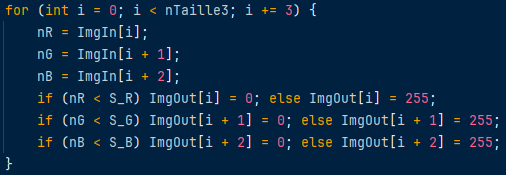
\includegraphics[width=.7\linewidth]{./out/test-couleur-code}}
		\caption{Code de \texttt{test\_couleur.cpp}}\label{Fig:test-couleur-code}
	\end{figure}

	On a utilis\'e l'image \emph{peppers.ppm} pour tester le programme avec des seuils à 80, 140 et 200 pour obtenir la
	transformation suivante :
	\begin{figure}[!htb]
		\begin{minipage}{0.48\textwidth}
			\centering
			\fbox{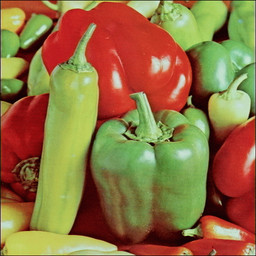
\includegraphics[width=.7\linewidth]{./out/orig-peppers}}
			\caption{Image originale}\label{Fig:orig-peppers}
		\end{minipage}\hfill
		\begin{minipage}{0.48\textwidth}
			\centering
			\fbox{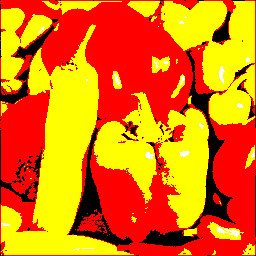
\includegraphics[width=.7\linewidth]{./out/test-couleur-peppers}}
			\caption{Image modifiée}\label{Fig:test-couleur-peppers}
		\end{minipage}
	\end{figure}

	\newpage
	\section{Histogrammes de 3 composantes d'une image couleur (ppm)}\label{sec:6}


	Pour cette partie, on a d\'evelopp\'e un programme \texttt{histo\_couleur.cpp} qui permet de g\'en\'erer
	l'histogramme d'une image ppm.
	Les données sont d'abord affichées dans la console, puis on les enregistre dans un fichier \texttt{histo-col.dat}
	pour pouvoir les visualiser avec \emph{gnuplot}.
	Le nom du fichier de sortie peut être rajouté en argument lors de l'exécution du programme.

	L'essentiel du code est le suivant : % insertion en image du code
	\begin{figure}[!htb]
		\centering
		\fbox{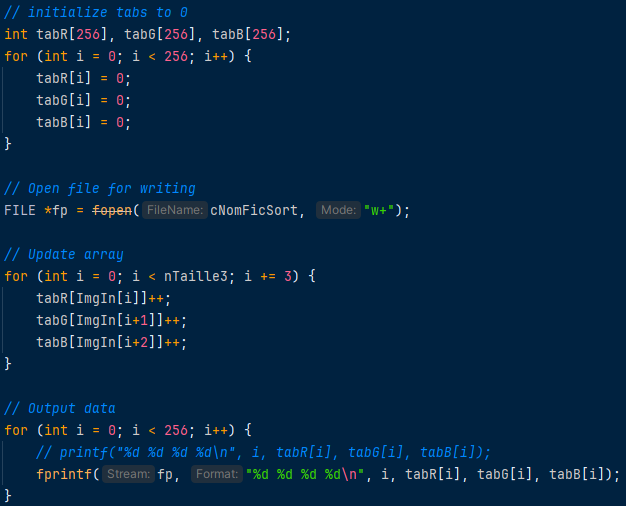
\includegraphics[width=.7\linewidth]{./out/histo-couleur-code}}
		\caption{Code de \texttt{histo\_couleur.cpp}}\label{Fig:histo-couleur-code}
	\end{figure}

	On a utilis\'e l'image \emph{peppers.ppm} pour tester le programme. Cela donne les r\'esultats suivants :
	% insert image of data file then of the histogram
	\begin{figure}[!htb]
		\begin{minipage}{0.48\textwidth}
			\centering
			% adjust image with height instead of width
			\fbox{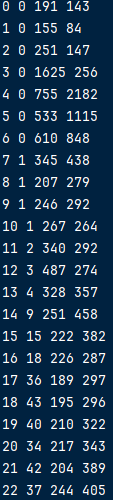
\includegraphics[height=0.7\linewidth]{./out/histo-couleur-data}}
			\caption{Donn\'ees de l'histogramme}\label{Fig:histo-couleur-data}
		\end{minipage}\hfill
		\begin{minipage}{0.48\textwidth}
			\centering
			\fbox{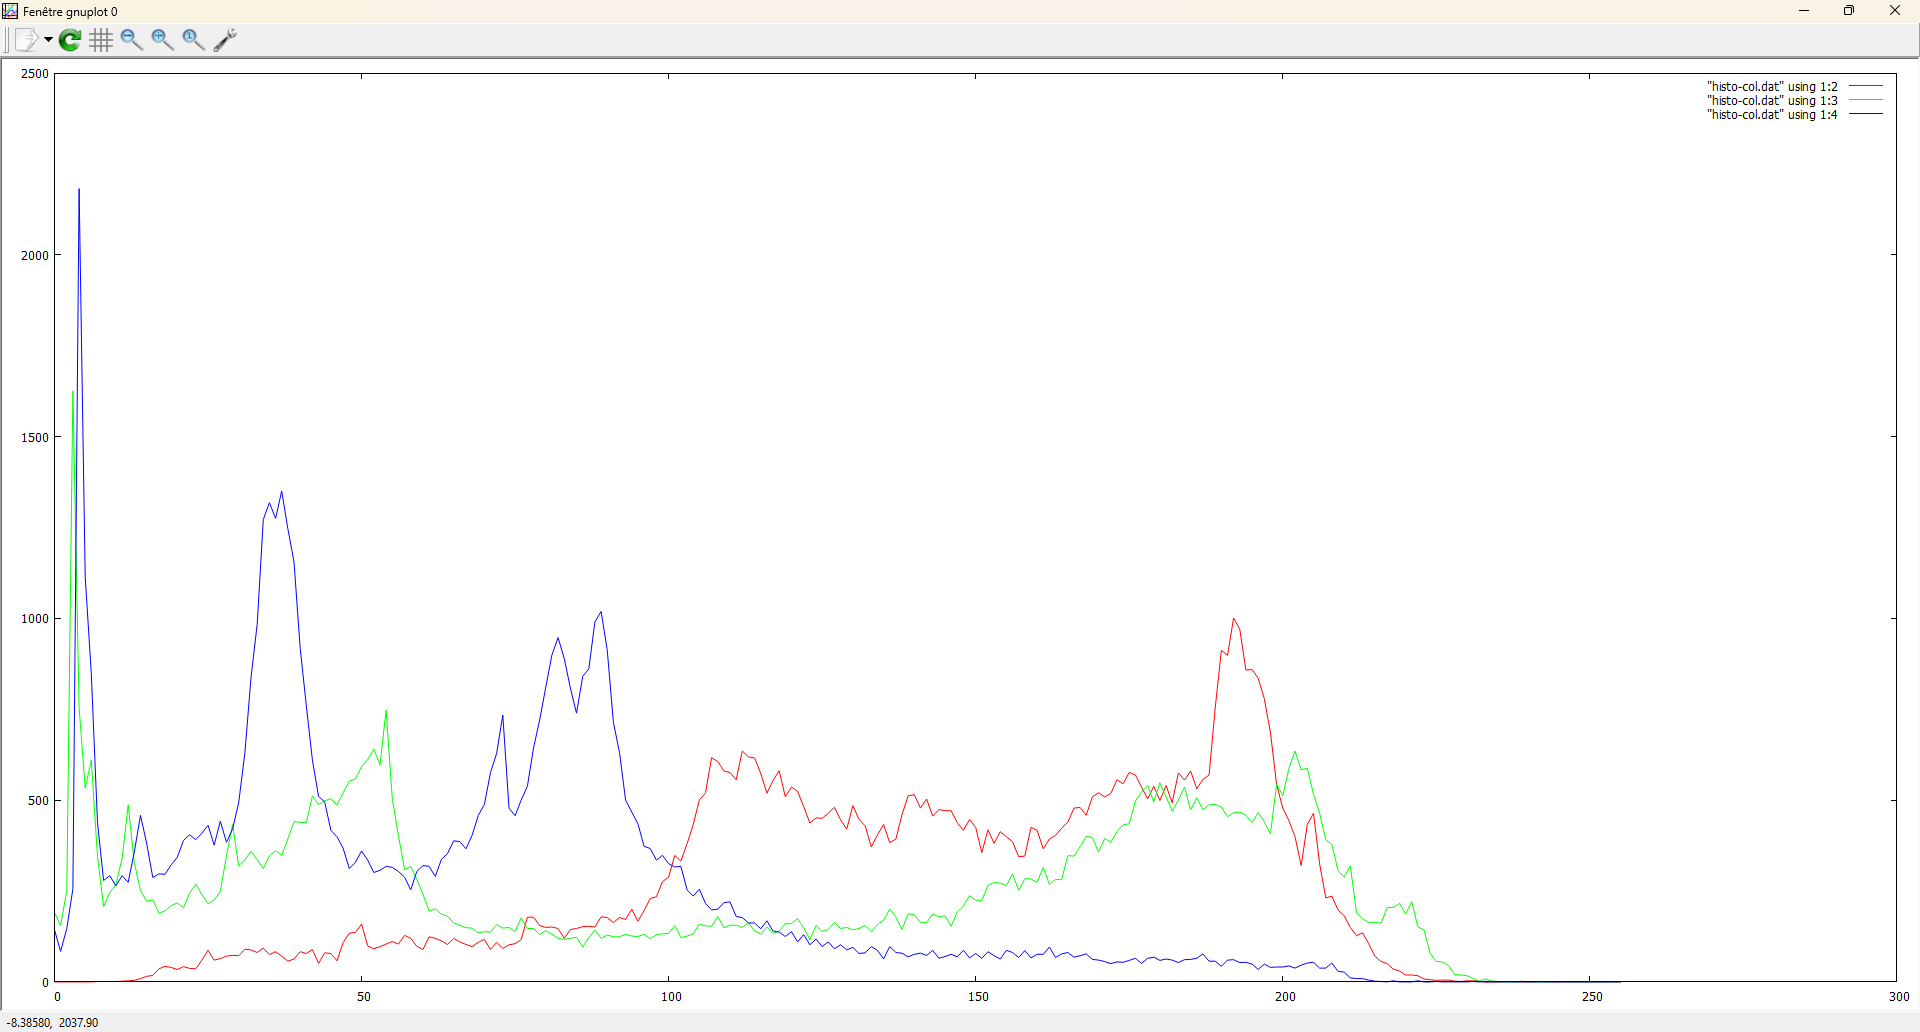
\includegraphics[width=.7\linewidth]{./out/histo-couleur-plot}}
			\caption{Histogramme de l'image}\label{Fig:histo-couleur-plot}
		\end{minipage}
	\end{figure}

	\newpage
	\section{Conclusion}\label{sec:7}
	Ce TP a permis de prendre en main une librairie de traitement d'images, en l'occurrence la librairie de William
	Puech.
	On a pu effectuer des seuillages sur des images au format pgm, puis sur des images au format ppm.
	On a aussi pu g\'en\'erer des histogrammes pour des images au format pgm, ensuite pour des images au format ppm.
	Enfin, on a pu g\'en\'erer des profils pour des images au format pgm.
\end{document}
